%%%%%%%%%%%%%%%%%%%%%%%%%%%%%%%%
% Section 3 (method+theory): 정의 -> exploration
%   -> annealing -> 성능 향상
% Formal derivations are deferred to Appendix~\ref{app:proofs}.
%%%%%%%%%%%%%%%%%%%%%%%%%%%%%%%%

\section{Random Soft Prompt와 작동 원리}\label{sec:why_rsp_works}

이 절은 논문에서 사용하는 핵심 메커니즘을 정리한다. rollout은 한 번 샘플한 RSP를 고정한 채 끝까지 수행한 자기회귀 디코딩 한 번을 뜻한다. 한 rollout 안에서 RSP는 attention을 통해 생성 초반의 next-token 결정을 흔들 수 있고, 캐시가 자라면 그 영향은 약해진다. rollout마다 RSP를 다시 뽑으면 그 분기 차이가 Pass@N 이득으로 누적될 수 있다. 본문에는 핵심 명제와 직관만 두고, 도출과 증명은 Appendix~\ref{app:proofs}로 보낸다.

% ================================================================
\subsection{Random Soft Prompt}\label{sec:rsp_definition}
% ================================================================

먼저 분석 대상부터 정리한다. 토큰 임베딩 행렬을 $\mathbf{W}_E \in \mathbb{R}^{V\times d}$로 두자($V$는 어휘 크기, $d$는 은닉 차원). 그 항별 평균과 표준편차를 $\mu_E := \tfrac{1}{Vd}\sum_{i,k}[\mathbf{W}_E]_{i,k}$, $\sigma_E := \mathrm{std}(\mathbf{W}_E)$라 하자. 길이 $L$의 RSP는 다음 분포에서 독립 추첨한 연속 벡터 시퀀스 $\mathbf{H} = [h_1,\dots,h_L]\in\mathbb{R}^{L\times d}$이다.
\begin{equation}\label{eq:rsp_def}
h_j \;\sim\; \mathcal{N}(\mu_E\mathbf{1}_d,\;\sigma_E^2\mathbf{I}_d), \quad j=1,\dots,L.
\end{equation}
중심화한 $\bar h_j := h_j - \mu_E\mathbf{1}_d \sim \mathcal{N}(0,\sigma_E^2\mathbf{I}_d)$은 평균 0의 등방 가우시안이다. 입력 임베딩 시퀀스 $\mathbf{X}$에는 prefix $[\mathbf{H};\mathbf{X}]$, infix, suffix $[\mathbf{X};\mathbf{H}]$ 세 방식 가운데 하나로 주입한다 \citep{kang2025model, xu2025softcot, ye2025thinking, zhang2025memgen}. 반복 샘플링 프로토콜에서는 비교하는 rollout들의 prompt 추첨과 디코딩 무작위성을 모두 독립으로 둔다.

무작위성의 목적은 임베딩 분포를 흉내 내는 데 있지 않다. 같은 텍스트 prompt를 여러 번 실행할 때 각 rollout이 \emph{독립적인} 섭동을 받도록 하는 데 있다. 탐색에 필요한 것은 바로 그 독립성이다.

% ================================================================
\subsection{Exploration: 왜 첫 몇 토큰이 움직이는가}\label{sec:improve}
% ================================================================

RSP가 초반에 영향을 줄 수 있는 이유는, 캐시가 아직 짧을 때는 무작위 토큰에도 무시할 수 없는 attention mass가 갈 수 있기 때문이다. self-attention 레이어 $\ell$이 실제 토큰 $n$개와 RSP 토큰 $L$개를 함께 attend하고, attention 가중치를 $\alpha_{ij}^{(\ell)}$, value 벡터를 실제 측과 RSP 측에서 각각 $\mathbf{v}_j^{(\ell)}$, $\mathbf{v}_{r_j}^{(\ell)}$라 하자. 이때 RSP 토큰에 배정된 attention mass를
\[
w_{r,i}^{(\ell)} := \sum_{j'=1}^{L} \alpha_{i,n+j'}^{(\ell)}
\]
로 두면 attention 출력은 정확히
\begin{equation}\label{eq:decomp}
\mathbf{x}_i^{(\ell+1)}
= (1-w_{r,i}^{(\ell)})\,\tilde{\mathbf{x}}_i^{(\ell+1)} + \boldsymbol{\eta}_i^{(\ell)},
\quad
\tilde{\mathbf{x}}_i^{(\ell+1)} := \sum_{j=1}^{n} \tfrac{\alpha_{ij}^{(\ell)}}{1-w_{r,i}^{(\ell)}}\mathbf{v}_j^{(\ell)},
\quad
\boldsymbol{\eta}_i^{(\ell)} := \sum_{j'=1}^{L} \alpha_{i,n+j'}^{(\ell)}\mathbf{v}_{r_{j'}}^{(\ell)}
\end{equation}
로 분해된다. 이는 근사가 아니라 대수적 항등식이다. 그리고 $\|\boldsymbol{\eta}_i^{(\ell)}\| \le w_{r,i}^{(\ell)} \max_{j'}\|\mathbf{v}_{r_{j'}}^{(\ell)}\|$이므로, \emph{같은 스칼라} $w_{r,i}^{(\ell)} \in [0,1]$가 실제 신호 감쇠와 무작위 기여 크기를 동시에 통제한다.

이제 남는 질문은 이 스칼라가 초반에 실제로 0에서 떨어져 있느냐다. 레이어 $\ell$에서 query를 $\mathbf{q}_i^{(\ell)}$, 실제와 RSP key를 각각 $\mathbf{k}_j^{(\ell)}$, $\mathbf{k}_{r_{j'}}^{(\ell)}$로 두자.

\begin{proposition}[초반 exploration의 lower envelope]\label{prop:lower_env}
역방향 logit gap을 $\Delta_i'^{(\ell)} := \max_{j\in[n]}(\mathbf{q}_i^{(\ell)})^\top\mathbf{k}_j^{(\ell)} - \min_{j'\in[L]}(\mathbf{q}_i^{(\ell)})^\top\mathbf{k}_{r_{j'}}^{(\ell)}$로 두면, scaled-dot-product attention에서
\[
w_{r,i}^{(\ell)} \;\ge\; \frac{L}{L + n\,\exp(\Delta_i'^{(\ell)}/\sqrt d)}
\]
가 성립한다.
\end{proposition}

증명은 softmax 부등식의 대칭형으로 Appendix~\ref{app:proofs}에 있다. Proposition~\ref{prop:lower_env}의 의미는 단순하다. 최악의 RSP token score가 best real-token score보다 너무 낮지 않다면, 생성 초반에는 무작위 토큰이 여전히 양의 attention mass를 받아 한 rollout 안에서 다른 초기 분기를 열 수 있다.

% ================================================================
\subsection{Annealing: 왜 효과가 사라지는가}\label{sec:converge}
% ================================================================

초반 영향을 만들었던 바로 그 스칼라가 후반에는 RSP를 사라지게 만든다. 정방향 logit gap을
\[
\Delta_i^{(\ell)} := \min_{j\in[n]}(\mathbf{q}_i^{(\ell)})^\top\mathbf{k}_j^{(\ell)} - \max_{j'\in[L]}(\mathbf{q}_i^{(\ell)})^\top\mathbf{k}_{r_{j'}}^{(\ell)},
\qquad
\Delta_i^{(\ell)} \le \Delta_i'^{(\ell)}
\]
로 두자.

\begin{theorem}[후반 어닐링의 upper envelope]\label{thm:decay}
scaled-dot-product attention에서
\[
w_{r,i}^{(\ell)} \;\le\; \frac{L}{L + n\,\exp(\Delta_i^{(\ell)}/\sqrt d)}
\]
가 성립한다. 우변은 $L$과 $\Delta_i^{(\ell)}$를 고정하면 $n$에 대해 엄격히 감소하고, $n\to\infty$이면 0으로 간다.
\end{theorem}

Proposition~\ref{prop:lower_env}와 결합하면 양방향 sandwich가 된다.
\begin{equation}\label{eq:sandwich}
\frac{L}{L+n\,\exp(\Delta_i'^{(\ell)}/\sqrt d)} \;\le\; w_{r,i}^{(\ell)} \;\le\; \frac{L}{L+n\,\exp(\Delta_i^{(\ell)}/\sqrt d)}.
\end{equation}
정리의 해석은 조심스럽다. 실현된 $w_{r,i}^{(\ell)}$가 step마다 반드시 단조 감소한다는 뜻은 아니다. query, key, hidden state가 함께 변하므로 두 gap도 계속 움직인다. 다만 \emph{같은 gap을 유지한다면}, 캐시 성장만으로 가능한 최대 RSP attention mass가 줄어든다는 뜻이다. Eq.~\eqref{eq:decomp}가 무작위 기여를 같은 스칼라로 묶어 두므로, perturbation도 이 fixed-gap envelope의 제약을 받는다. 전체 블록을 통한 유한 깊이 전파 제어는 Appendix~\ref{app:proofs}에 정리한다.

\begin{figure}[ht]
  \centering
  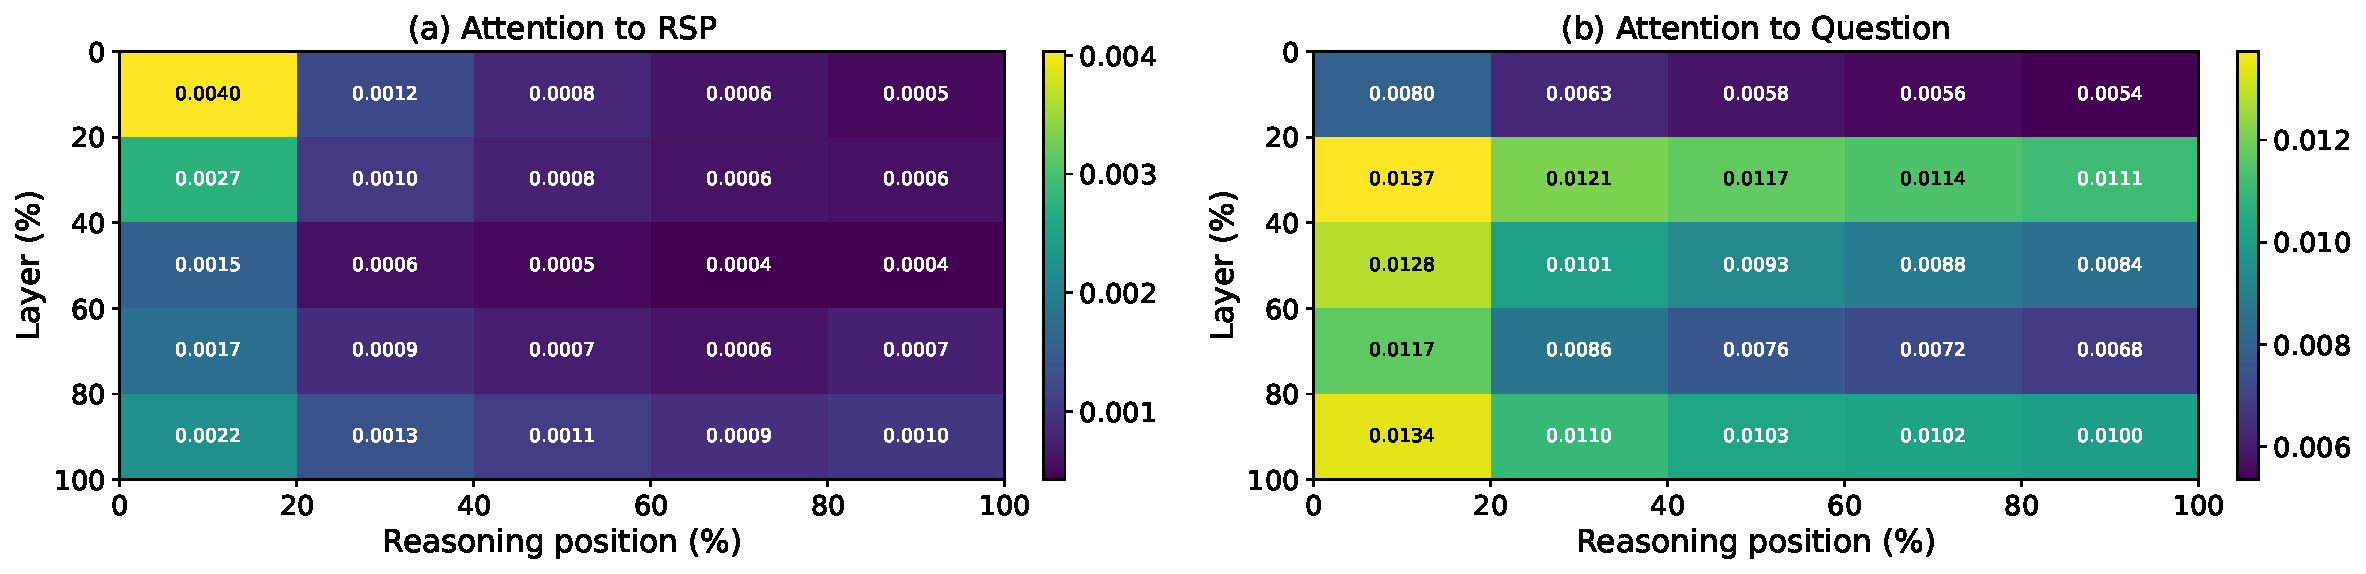
\includegraphics[width=0.72\textwidth]{img/attention/heatmap_qwen7b_suffix.pdf}
  \caption{Qwen2.5-Math-7B의 토큰별 attention 질량(suffix, MATH-500 500문제, 문제마다 독립 RSP). (a) RSP 토큰 attention은 추론 위치 축에서 감소하며 Eq.~\eqref{eq:sandwich}와 맞는다. 레이어 축의 추가 감소는 깊은 레이어가 real-vs-random gap을 더 날카롭게 만든다는 별도 경험적 현상이지, Theorem~\ref{thm:decay}만의 직접 귀결은 아니다. (b) 질문 토큰 attention은 비교적 균일하게 유지된다. 보고한 양은 Appendix~\ref{app:attention_mass}의 per-token mass로, $w_{r,i}^{(\ell)}/L$을 head와 sample에 대해 평균한 값이다.}
  \label{fig:attention_mass}
\end{figure}

% ================================================================
\subsection{성능 향상: 왜 독립 재실행이 도움이 되는가}\label{sec:multipath}
% ================================================================

앞의 두 envelope은 한 rollout 안에서 RSP가 얼마나 움직일 수 있는지를 설명했다. 이제 남는 질문은 성능이다. 왜 \emph{새로운} RSP로 다시 실행할 때, 하나의 고정된 prompt를 반복하는 것보다 이득이 커질 수 있는가? 여기에는 prompt 분포에 대한 사실 하나와, 열린 branch가 실제로 정답에 도움이 되는지에 대한 별도의 task-side 사실 하나가 필요하다.

먼저 분포 쪽 사실부터 보자. 위 attention 항등식과 gap 부등식은 등방성을 요구하지 않지만, branch opening은 현재 prompt에 중요한 방향을 미리 편들지 않는 분포를 선호한다.

\begin{theorem}[방향 무관 미니맥스 커버리지]\label{thm:minimax_directional_coverage}
$\mathbb{R}^d$ 위 평균 0 분포 $D$가 분산 예산 $\mathrm{tr}(\Sigma_D)\le\rho^2$를 만족하면
\[
\min_{\|b\|=1}\mathrm{Var}_{h\sim D}(b^\top h) = \lambda_{\min}(\Sigma_D) \le \rho^2/d
\]
이고, 등호는 $\Sigma_D = (\rho^2/d)\mathbf{I}_d$일 때에만 성립한다.
\end{theorem}

등호에 필요한 핵심은 가우시안 그 자체가 아니라 등방 공분산이다. 여기서 가우시안을 택한 이유는 둘째 성질 때문이다. 가우시안 법칙은 모든 비공집합 열린집합에 양의 확률을 부여하므로, 2차 모멘트 수준에서 특정 방향을 미리 편들지 않으면서도 국소적인 branch-opening 영역을 배제하지 않는다(Proposition~\ref{prop:gaussian_open_support}).

이제 centered prompt $\bar h = 0$ 주변에서 next-token logit의 1차 affine surrogate를
\[
z_i^{\mathrm{lin}}(\bar h) := z_i + a_i^\top \bar h,
\qquad
a_i := \nabla_{\bar h} z_i(0)
\]
로 둔다. baseline에서 제외된 토큰 $i$의 top-$K$ 진입 영역은
\[
\mathcal{G}_{i,K}
\;:=\;
\bigl\{\bar h \in \mathbb{R}^d : \#\{j\neq i : z_j^{\mathrm{lin}}(\bar h) > z_i^{\mathrm{lin}}(\bar h)\} \le K-1\bigr\}
\]
로 쓸 수 있다.

\begin{proposition}[조건부 top-$K$ 진입]\label{prop:support_expansion}
$\mathcal{G}_{i,K}$가 비공집합 열린집합을 포함하면, 등방 가우시안 prompt 법칙이 그 영역에 양의 확률을 부여하므로
\[
\mu_i := \Pr_{\bar h}(\bar h \in \mathcal{G}_{i,K}) > 0
\]
이다.
\end{proposition}

Proposition~\ref{prop:support_expansion}이 설명하는 메커니즘은 의도적으로 제한적이다. branch가 열릴 수 있다는 뜻이지, 열린 branch가 유용하다는 뜻은 아니다. 이를 task accuracy로 연결하려면 task-side 가정을 따로 둬야 한다. 문제 $x$에 대해 (M1) 각 독립 RSP 실행이 정답 trajectory에 도달할 주변 확률이 적어도 $p_{\min}(x)>0$이고, (M2) $N$번의 실행이 서로 독립이라고 하자.

\begin{proposition}[다중 경로 Pass@N]\label{prop:multi_path}
(M1)--(M2) 아래에서, $N$개의 독립 RSP 실행은
\[
\Pr\!\big(\mathrm{Pass@}N\text{ on }x\big) \;\ge\; 1-(1-p_{\min}(x))^N \;\ge\; 1-\exp(-N\,p_{\min}(x))
\]
를 만족한다.
\end{proposition}

이 역할 분담이 이 절의 핵심 해석이다. 메커니즘은 baseline 밖 후보를 \emph{후보권 안으로 들이는 것}까지만 책임진다. 들인 branch가 실제로 \emph{생산적}인지는 task의 성질에 달려 있으므로 $p_{\min}(x)>0$ 가정이 따로 필요하다. 같은 RSP를 모든 sample이 공유하면 누적 이득이 사라지는 이유도 여기 있다. 독립 재추첨이 없으면 branch를 다시 여는 것이 아니라 같은 branch를 반복 방문하게 되기 때문이다. §\ref{sec:experimental_analysis}는 바로 이 서명을 실험적으로 확인한다.
